\documentclass[11pt,a4paper]{article}
\usepackage[margin=2.5cm]{geometry}
\usepackage{amsmath,amssymb,graphicx,booktabs,float,setspace,placeins}
\usepackage[authoryear,round]{natbib}
\usepackage[hidelinks]{hyperref}
\onehalfspacing
\widowpenalty=10000
\clubpenalty=10000
\graphicspath{{figures/}}
\title{A log-Gaussian Cox model for latent river breeding sites and onchocerciasis prevalence}
\author{}
\date{10 November 2026}

\begin{document}
\maketitle

\section{Introduction}

Blackfly breeding sites are unobserved in the village prevalence data. We represent them by a log-Gaussian Cox process (LGCP) on the river network: a Gaussian field determines the local density of breeding sites, and each realized site contributes exposure to every village within its dispersal range. The same latent sites therefore link the village outcomes. This construction distinguishes uncertainty about where sites occur from variation in the intensity that generates them.

This report follows the data--model--estimation--results structure of the existing river-model reports. It describes the implemented LGCP, summarizes the full-data and spatial holdout analyses saved on 7 November 2026, and records the code improvements and validation performed on 10 November. The archived chains show substantial disagreement, including different regimes for the dispersal width. Their numerical summaries describe the saved simulations; a definitive comparison of converged Bayesian models remains unavailable.

A separate four-chain diagnostic run on 10 November records latent-field trajectories for the tail-down model at 800~km. This supplements the archived parameter diagnostics and leaves the original forecast comparisons unchanged.

\section{Data and spatial representation}

The analysis contains 900 REMO surveys in Sudan and South Sudan, with 2,386 positives among 37,831 individuals examined; 550 villages have no positives. The observed positive fraction is 6.31\%, and 24 villages have at least half their participants positive. The HydroRIVERS network retains reaches with average discharge at least 0.1~m$^3$/s. The saved design contains 286,068 river quadrature cells and 145,329 field vertices. At the 60~km dispersal cutoff, 68,980 cells can contribute to at least one survey.

The five breeding covariates are log discharge, log-transformed slope, capped log-transformed inundation, longitude and latitude. Each is centered and scaled using river-cell lengths as weights. Village transmission uses standardized log aridity; the occurrence regression uses aridity centered at 0.4 and divided by 0.2. These transformations are fixed in the archived design. The response and trial count of a held-out survey are both masked during fitting, while its original trial count is restored for predictive scoring.

\section{Model}\label{sec:model}

\subsection{Latent sites and their strengths}

Let $\Gamma$ denote the river network and $s_j$ the midpoint of cell $j$, whose length is $\ell_j$~km. Let $z_j$ contain its five breeding covariates, $\theta$ their coefficients, and $u_j$ the field interpolated from the graph vertices. Conditional on this field, the implemented cell model is
\[
 N_j\mid u_j,\theta\sim\operatorname{Poisson}(\mu_j),\qquad
 \mu_j=\ell_j\rho_0\exp(z_j^\top\theta+u_j),\qquad \rho_0=0.04\ \mathrm{km}^{-1},
\]
with conditionally independent cell counts. The baseline source rate is fixed and there is no breeding intercept in these analyses. The Gaussian field has either the symmetric Whittle--Mat\'ern precision or the tail-down precision supplied by the package, with field-scale parameter $\sigma_u=0.5$ and river-network range $r\in\{200,400,800\}$~km. The same field-scale parameter need not give identical marginal variances for the two graph constructions, particularly near junctions and boundaries.

Each site independently has strength $1-d$ or $1+d$ with equal probability. If $H_j\mid N_j\sim\operatorname{Binomial}(N_j,1/2)$ is the number of stronger sites in a cell, its total marked mass is
\[
 M_j=(1-d)(N_j-H_j)+(1+d)H_j.
\]
A site's strength is shared by all the villages it reaches. Its mean strength is one for every $d$, and the unit-strength model is obtained at $d=0$.

\subsection{Dispersal and village outcomes}

Let $x_i$ be the location of village $i$. The Gaussian dispersal kernel uses straight-line distance $h$, width $b$ and fixed cutoff $\phi=60$~km. With $\Phi$ denoting the standard normal distribution function, the line-normalized kernel and the village exposure are
\[
 K_b(h)=\frac{\exp\{-h^2/(2b^2)\}}
 {\sqrt{2\pi}\,b\{\Phi(\phi/b)-\Phi(-\phi/b)\}}\,\mathbf{1}\{h<\phi\},
 \qquad E_i=\sum_j K_b(\|x_i-s_j\|)M_j.
\]
Cell length enters the Poisson mean once; it does not multiply a site's kernel contribution again. The width $b$, cutoff $\phi$ and river-field range $r$ describe different scales. The package also supports a compact Wendland kernel, but the six archived comparisons in this report all use the Gaussian kernel.

Let $A_i$ indicate whether village $i$ is in an active transmission zone. Write $c_i=(\mathrm{AI}_i-0.4)/0.2$ for centered aridity and $v_i$ for standardized log aridity. In the archived analyses,
\begin{align*}
 A_i\mid E_i&\sim\operatorname{Bernoulli}(q_i), &
 \operatorname{logit}(q_i)&=\gamma_0+\gamma_c c_i+\gamma_E E_i,\\
 Y_i\mid A_i,E_i&\sim\operatorname{Binomial}(n_i,A_i p_i), &
 \operatorname{logit}(p_i)&=\log E_i+\beta_0+\beta_v v_i.
\end{align*}
Here $n_i$ is the number examined and $Y_i$ the number positive. A zero exposure gives $p_i=0$ exactly, although $q_i$ may remain positive. The occurrence indicator is shared by everyone in a village, so its marginal zero probability is
\[
 \Pr(Y_i=0\mid E_i)=1-q_i+q_i(1-p_i)^{n_i}.
\]
The package's alternative complementary log-log link sets $p_i=1-\exp\{-E_i\exp(\beta_0+\beta_v v_i)\}$. It is supported and tested, but is not the link used in the archived tables.

\subsection{Priors and interpretation}

All breeding, transmission and occurrence coefficients have independent $N(0,1.5^2)$ priors; $d$ is uniform on $[0,1]$, and $\log b$ is uniform on $[\log 1,\log 240]$, with $b$ measured in kilometres. The source rate, field scale, river range and cutoff are fixed within each model configuration. Thus uncertainty in these quantities is not included in the reported intervals. In particular, the inferred number of sites and their strength contrast depend on the assumed reference source rate. With prevalence alone, they should be interpreted as features of a latent exposure model rather than as directly measured breeding-site abundance.

\section{Estimation and approximations}

Estimation uses Markov chain Monte Carlo (MCMC) to explore the joint posterior of the breeding sites, the river field and the regression parameters. The observations constrain the sites through the exposure they generate, while the sites constrain the field through their Poisson intensities. We describe the marked Gaussian-kernel model with occurrence and \texttt{block\_slice} field updates used in the reported analyses.

\subsection{Posterior target and order of updates}

Write $g$ for the vector of field values at graph vertices and $W$ for the interpolation matrix, so that the cell field introduced above is $u_j=(Wg)_j$. Its prior is $g\sim N(0,Q^{-1})$, with the precision $Q$ fixed by the chosen field, range and scale. Let $\beta=(\beta_0,\beta_v)^\top$, $\gamma=(\gamma_0,\gamma_c,\gamma_E)^\top$, and $t=\log b$. We retain counts $N_j$ and $H_j$ only in the set $\mathcal J$ of cells within the cutoff of at least one supplied village. The remaining counts integrate out conditional on the field; the field itself remains defined on the full graph.

Let $\mathcal I$ denote the training villages and write $E=E(N,H,d,e^t)$. With $p_i=p_i(E_i,\beta)$ and $q_i=q_i(E_i,\gamma)$ as defined in Section~\ref{sec:model}, the augmented village likelihood is
\begin{equation}\label{eq:augmented-village}
 L_{\mathrm v}(E,\beta,\gamma;A)
 =\prod_{i\in\mathcal I}
 q_i^{A_i}(1-q_i)^{1-A_i}
 \operatorname{Bin}(y_i;n_i,A_i p_i),
\end{equation}
where $\operatorname{Bin}(k;n,p)$ denotes a binomial probability mass. If $\psi=(g,\theta,\beta,\gamma,N,H,A,d,t)$ and $\pi_0$ is the joint prior density of its continuous components, the posterior target is
\begin{equation}\label{eq:lgcp-posterior}
 \pi(\psi\mid y)\ \propto\
 L_{\mathrm v}(E,\beta,\gamma;A)\,
 \prod_{j\in\mathcal J}
 \left\{\operatorname{Pois}(N_j;\mu_j)
        \operatorname{Bin}(H_j;N_j,1/2)\right\}
 \pi_0(g,\theta,\beta,\gamma,d,t).
\end{equation}
Here $\operatorname{Pois}(k;\mu)$ denotes a Poisson mass and $\pi_0$ combines the Gaussian priors with the uniform priors for $d$ and $t$. The density in Equation~\eqref{eq:lgcp-posterior} is expressed in log width $t$; a density expressed in width $b$ would instead contain the prior factor $1/b$ on its support.

One sweep updates $A$, then $\gamma$, then the counts and their locations, followed by $d$, $t$ when scheduled, $\theta$, $g$, and finally $\beta$. All other components are held at their current values within an update. Initialization places at least one site in reach of every positive village, reusing a site when it already reaches several positive villages. This supplies a configuration with positive survey likelihood rather than starting from an impossible empty landscape.

\subsection{Village activity and the point pattern}

The activity update is an exact Bernoulli draw. A positive observation requires $A_i=1$. For a training village with $y_i=0$, Bayes' rule gives
\[
 \Pr(A_i=1\mid y_i=0,E_i,\beta,\gamma)
 =\frac{q_i(1-p_i)^{n_i}}
 {1-q_i+q_i(1-p_i)^{n_i}}.
\]
Thus a zero can be explained either by an inactive village or by no positives among the people examined in an active village. Given $A$ and $E$, updating $\gamma$ is a logistic regression with responses $A_i$ and predictors $(1,c_i,E_i)$. The corrected Gaussian and slice updates for its coefficients are described below.

The count sweep visits cells in a random order. For a selected cell, it proposes
\[
 N_j'\sim\operatorname{Poisson}(\mu_j),\qquad
 H_j'\mid N_j'\sim\operatorname{Binomial}(N_j',1/2).
\]
The reported runs refresh one cell at a time; the implementation also permits joint refreshes of several cells. These proposals are drawn from the conditional count and mark priors appearing in Equation~\eqref{eq:lgcp-posterior}. Their forward and reverse proposal factors therefore cancel the corresponding prior ratio in the Metropolis--Hastings rule \citep[Section~2.2]{hastings1970}. The acceptance probability reduces to
\begin{equation}\label{eq:count-acceptance}
 \alpha=\min\left\{1,
 \frac{L_{\mathrm v}(E',\beta,\gamma;A)}
      {L_{\mathrm v}(E,\beta,\gamma;A)}\right\},
\end{equation}
where $E'$ is the exposure from the proposed pattern. Both the infection likelihood and the occurrence likelihood enter this ratio because $q_i$ depends on exposure. Removing the last source that reaches a positive village makes its likelihood zero and rejects the proposal. Only villages reached by changed cells need to be reevaluated.

Relocation proposals complement count refreshes. They select an existing labelled site and propose a new cell within its current spatial tile, with probability proportional to $\mu_j$ over that tile, retaining its weak or strong type. Conditional on the tile's site count and types, these are the prior location probabilities, so the acceptance rule again has the likelihood-ratio form in Equation~\eqref{eq:count-acceptance}. The tiles shift between sweeps. This permits a source to move while preserving total marked mass, without requiring a separate deletion followed by a birth.

\subsection{Mark spread and dispersal width}

Given $N$ and $H$, exposure is affine in the spread:
\[
 E_i(d)=(1-d)\sum_j K_b(\|x_i-s_j\|)(N_j-H_j)
       +(1+d)\sum_j K_b(\|x_i-s_j\|)H_j.
\]
The uniform prior on $d\in[0,1]$ leaves a one-dimensional likelihood target. We use the slice construction of \citet[Section~4]{neal2003}: draw $U\sim\operatorname{Uniform}(0,1)$ and set the log threshold to $\log L_{\mathrm v}(E(d),\beta,\gamma;A)+\log U$. Candidates are drawn from an interval initially equal to $[0,1]$; a rejected candidate shortens the interval on its side of the current $d$, until the candidate likelihood exceeds the threshold.

The width update proposes $t'=t+\varepsilon$, with $\varepsilon\sim N(0,s_t^2)$, and rejects values outside $[\log 1,\log 240]$. The proposal is symmetric and the prior is uniform in $t$, so an in-bounds proposal again uses the village likelihood ratio, now recomputing the normalized kernel and exposure at $b'=e^{t'}$. There is no additional Jacobian in this coordinate. The cutoff remains fixed, so changing width does not add or remove cells from $\mathcal J$. A proposal is attempted every fourth sweep; $s_t$ is adjusted during burn-in toward an acceptance fraction of 0.35 and then held fixed.

\subsection{Conditional Poisson field and regression updates}

The field update exploits the augmentation by site counts. Once the point pattern and village parameters are fixed, the village likelihood contains neither $g$ nor $\theta$. Write $Z$ for the matrix with rows $z_j^\top$ for $j\in\mathcal J$, and set
\[
 \eta_j=\log(\ell_j\rho_0)+z_j^\top\theta+(Wg)_j,
 \qquad \mu_j=e^{\eta_j}.
\]
With regression prior standard deviation $\tau=1.5$, the conditional log posterior of $(g,\theta)$, up to a constant, is
\begin{equation}\label{eq:poisson-field-target}
 \sum_{j\in\mathcal J}\{N_j\eta_j-e^{\eta_j}\}
 -\tfrac12g^\top Qg-\frac{\theta^\top\theta}{2\tau^2}.
\end{equation}
The surveys inform the field through the currently imputed counts. A second binomial factor must not be introduced into this conditional update.

First, $\theta$ is updated with $g$ fixed. The score and negative Hessian of its conditional log posterior are
\[
 s_\theta=Z^\top(N-\mu)-\theta/\tau^2,
 \qquad
 H_\theta=Z^\top\operatorname{diag}(\mu)Z+\tau^{-2}I.
\]
The proposal is Gaussian with mean $\theta+H_\theta^{-1}s_\theta$ and covariance $H_\theta^{-1}$. To state the correction for this and the village regressions, let $a$ denote the coefficient block being updated, $f(a)$ its conditional posterior density, and $r(a'\mid a)$ the Gaussian proposal formed at $a$. We accept with probability
\begin{equation}\label{eq:regression-acceptance}
 \min\left\{1,
 \frac{f(a')\,r(a\mid a')}{f(a)\,r(a'\mid a)}\right\}.
\end{equation}
The reverse density is formed using the score and Hessian at $a'$, including its Gaussian normalizing constant. This implements the asymmetric-proposal correction of \citet[Section~2.2]{hastings1970}; the Newton step specifies a proposal mean, not a deterministic replacement of the coefficients by an optimizer.

Next, the field is updated conditionally on the new $\theta$. For a vertex block $B$, let $C$ denote its complement. Completing the square in the Gaussian prior gives
\[
 g_B\mid g_C\sim N(m_B,Q_{BB}^{-1}),\qquad
 m_B=-Q_{BB}^{-1}Q_{BC}g_C.
\]
We apply elliptical slice sampling \citep[Section~2 and Figure~2]{murray2010} to the centered block $g_B-m_B$, with an independent $\nu_B\sim N(0,Q_{BB}^{-1})$. Candidate fields lie on the ellipse
\[
 g_B'=m_B+(g_B-m_B)\cos\omega+\nu_B\sin\omega.
\]
A random log-likelihood threshold is formed from the current Poisson likelihood. The initial angle is uniform on $[0,2\pi]$ and defines a bracket $[\omega-2\pi,\omega]$. Rejected angles shrink this bracket while retaining zero, until the candidate exceeds the threshold. The Gaussian prior is handled by the ellipse; only the first sum in Equation~\eqref{eq:poisson-field-target} enters the slice test.

For the two field types used here, the implementation partitions vertices into two colours. Different connected blocks of one colour have no precision links and no cell projects onto two such blocks. Their conditional targets therefore separate given the other colour, $N$ and $\theta$, allowing an angle for each block. Both colours are updated, and the band boundaries alternate between two partitions. Since $Q$ is fixed, the sparse conditional Cholesky factors can be computed once and reused.

This is a blocked slice-within-Gibbs scheme: the vertices in a connected block move jointly while the remaining field is fixed. One elliptical slice transition preserves the block's conditional posterior; it does not draw independently from that non-Gaussian conditional distribution. The bands span 12 graph-edge steps, with a six-step shift between partitions. Among blocks touching the survey footprint, the median size is nine vertices in both partitions, and the largest blocks have 66 and 90 vertices, respectively. These local updates make it necessary to check broad spatial field summaries as well as individual coordinates; Section~\ref{sec:field-mixing} reports that check.

Finally, $\beta$ is updated by logistic regression on the active training villages, using $\log E_i$ as a known offset. The occurrence regression for $\gamma$ uses the activity labels instead. Both use the corrected local Gaussian proposal above on three sweeps out of four and a Gaussian-prior elliptical slice update on the fourth sweep in these runs. Inactive villages have no infection-likelihood contribution, but their occurrence labels still contribute to the $\gamma$ regression.

\subsection{Alternative field proposals, summaries and convergence}

Two alternative field updates are available. The global \texttt{slice} option updates the joint vector $(\theta,g)$ on an ellipse defined by its Gaussian prior. The \texttt{laplace} option finds the mode and negative Hessian of Equation~\eqref{eq:poisson-field-target}, draws from the resulting Gaussian approximation, and applies the independence Metropolis--Hastings correction. This Gaussian serves as a proposal; approximation error is accounted for in the acceptance ratio. The reported runs use the conditional block method described above.

After burn-in, the retained states provide posterior summaries of coefficients, site counts, occupation probabilities and village prevalence. For example, with $S$ retained states, the prevalence estimate is $S^{-1}\sum_{s=1}^S A_i^{(s)}p_i^{(s)}$, preserving the dependence between activity and infection risk. A held-out village contributes neither factor in Equation~\eqref{eq:augmented-village}; its predictive activity is generated from $q_i$ at the sampled exposure, without conditioning on its omitted outcome.

Full-data analyses used four 8,000-sweep chains per configuration, discarding 2,000 sweeps from each; initial widths were 10, 20, 40 and 80~km. Each spatial holdout refit used four 12,000-sweep chains, discarding 6,000. We assess agreement and simulation efficiency using rank-normalized $\widehat R$ and bulk ESS \citep{vehtari2021}. The reported screening thresholds, $\widehat R>1.05$ or ESS below 100, reproduce the archived analysis; they are not a claim that all unflagged estimates are accurate. In particular, \citet[Section~2]{vehtari2021} recommend the stricter $\widehat R<1.01$ and checking Monte Carlo errors for the quantities of interest.

The cell-midpoint representation and field interpolation define a spatial approximation, while finite MCMC length introduces simulation error within that model. All inference is conditional on the specified source rate, field scale, river range and cutoff. Valid update formulas and favorable acceptance rates do not establish adequate exploration of the joint posterior; the observed chain disagreement remains a limitation of the reported estimates.


\section{Predictive assessment}

The five spatial folds each contain 180 villages, with 100~km blocks assigned together. Training and test blocks can touch: there is no geographic buffer. Each held-out predictive distribution averages $\operatorname{Binomial}(n_i,A_i p_i)$ over the retained joint draws from the corresponding training fit. Field range and other fixed settings remain as specified above, while the width and regression coefficients are fitted separately in every fold.

We report the Brier score for the event of zero positives, the continuous ranked probability score (CRPS) for the observed fraction positive, and the sum of village marginal count log scores. Brier and CRPS give equal weight to villages, and lower values are better; higher count log scores are better. The sum of marginal log scores is not a joint spatial log likelihood. The expected number of nonzero villages provides an additional calibration summary.

The full-data checks answer a separate question. Each configuration generated 2,000 fresh river landscapes: a new field, sites, marks, village activities and outcomes, with parameter draws taken jointly from the fitted chains. These simulations use the observed locations and sample sizes, but regenerate the local field and sites instead of conditioning on the inferred local landscape. They assess the model's capacity to generate the observed overall pattern; their scores are not held-out validation scores.

\section{Results}

\subsection{Spatial holdout forecasts}

Table~\ref{tab:cv} and Figure~\ref{fig:scores} summarize the saved forecasts. Tail-down at 800~km has the smallest Brier and CRPS and the largest count log score in this finite-chain comparison. The expected nonzero counts are close to the observed 350 across configurations. These rankings are provisional because all 30 model--fold combinations fail the recorded convergence criteria, discussed below.

\begin{table}[H]
\centering\small
\caption{Five-fold held-out scores from the archived runs. Each row uses all 900 villages exactly once as held-out observations.}
\label{tab:cv}
\begin{tabular}{lrrrrr}
\toprule
Field & $r$ (km) & Brier & CRPS & Log score & Nonzero\\
\midrule
Whittle--Mat\'ern & 200 & 0.1088 & 0.0432 & -1454.6 & 344.7 \\
Tail-down & 200 & 0.1032 & 0.0405 & -1360.7 & 347.4 \\
Whittle--Mat\'ern & 400 & 0.1069 & 0.0420 & -1399.0 & 346.0 \\
Tail-down & 400 & 0.1022 & 0.0406 & -1381.9 & 347.6 \\
Whittle--Mat\'ern & 800 & 0.1060 & 0.0424 & -1368.7 & 350.9 \\
Tail-down & 800 & 0.1005 & 0.0399 & -1337.0 & 347.1 \\
\bottomrule

\end{tabular}
\end{table}

\begin{figure}[htbp]
\centering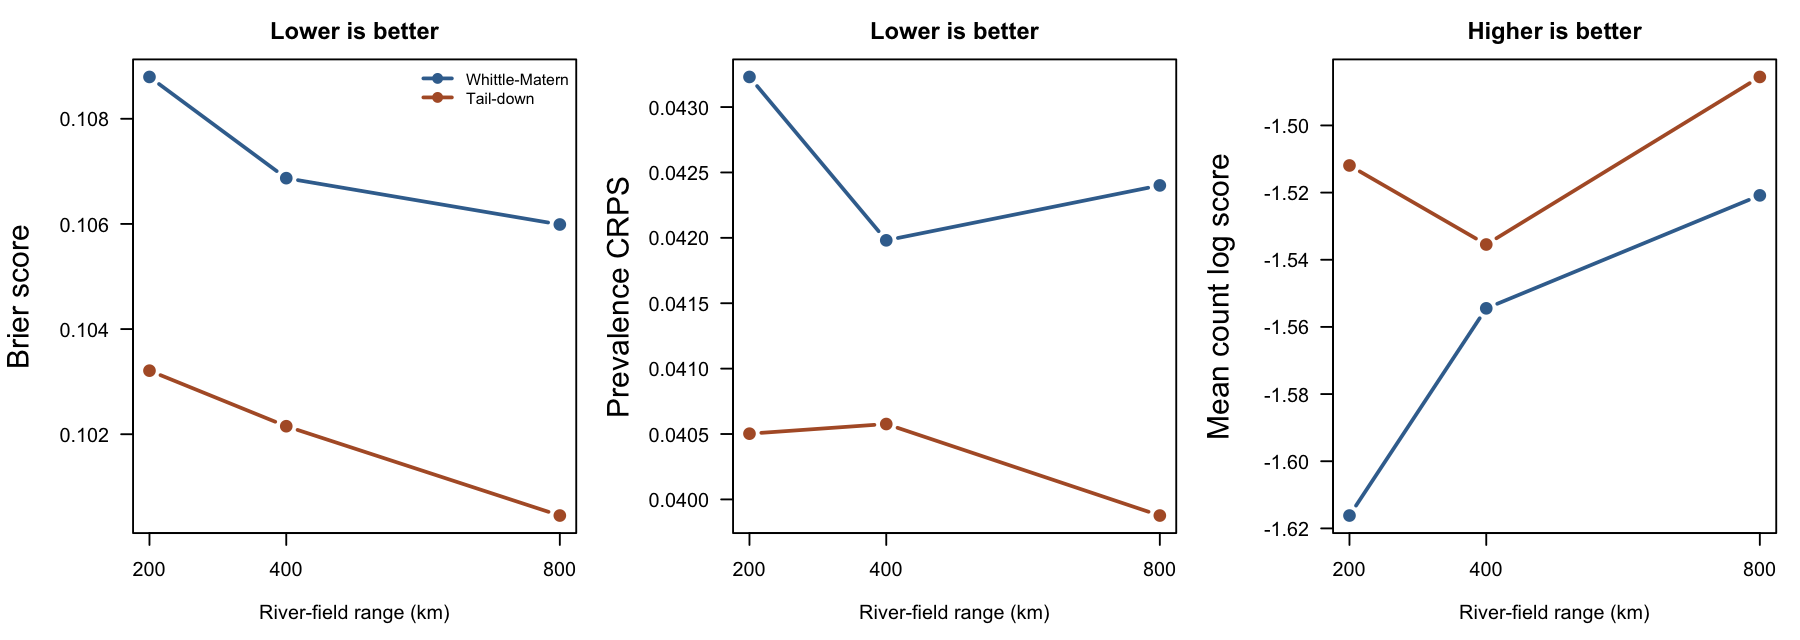
\includegraphics[width=\textwidth]{heldout_scores.png}
\caption{Scores of the saved held-out forecasts by field and river range. The log score is shown per village; all configurations have convergence flags.}
\label{fig:scores}
\end{figure}

Figure~\ref{fig:map} compares observed proportions with held-out mean prevalence for the tail-down 800~km configuration. The predictions show the broad north--south contrast, with less local variation than the observed fractions. They are forecasts at survey locations; combining their five fitted folds does not produce a single joint realization of the river process.

\begin{figure}[htbp]
\centering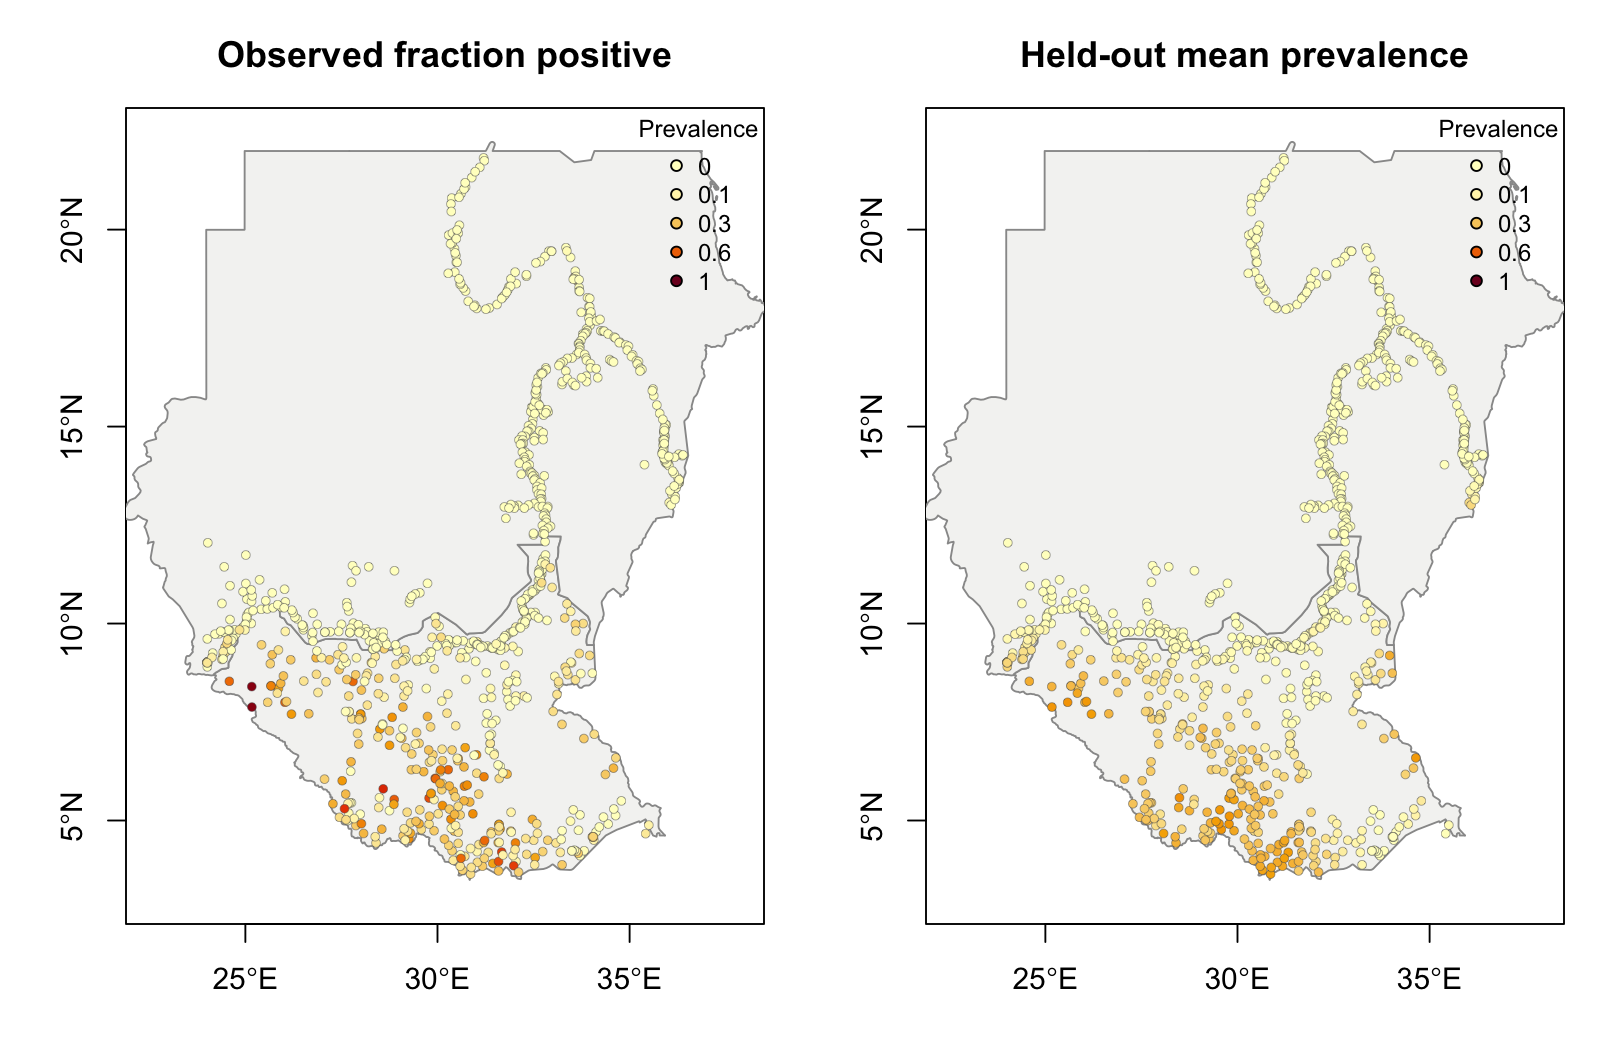
\includegraphics[width=.93\textwidth]{heldout_map.png}
\caption{Observed fractions and held-out mean prevalence at the 900 surveys, with a common color scale. The right panel uses tail-down at 800~km and combines predictions from five training fits.}
\label{fig:map}
\end{figure}

\subsection{Chain agreement and predictive stability}

We use rank-normalized $\widehat R$ to summarize between-chain agreement and bulk effective sample size (ESS) to summarize information in the retained draws \citep{vehtari2021}. The archived diagnostic flag is any non-finite diagnostic, parameter $\widehat R>1.05$, or bulk ESS below 100. Every holdout configuration has all five folds flagged. Table~\ref{tab:diagnostics} also reports how many held-out village risks have poor diagnostics; agreement of a few aggregate scores does not establish agreement of the local predictions.

\begin{table}[H]
\centering\small
\caption{Diagnostics across the five holdout fits. The first two diagnostic columns are the worst monitored parameter values; the last two count held-out village-risk flags.}
\label{tab:diagnostics}
\begin{tabular}{lrrrrr}
\toprule
Field & $r$ (km) & Max $\widehat R$ & Min ESS & Risk $\widehat R>1.05$ & Risk ESS $<100$\\
\midrule
Whittle--Mat\'ern & 200 & 1.73 & 6.3 & 47/900 & 31/900 \\
Tail-down & 200 & 2.27 & 5.1 & 151/900 & 133/900 \\
Whittle--Mat\'ern & 400 & 1.97 & 5.5 & 104/900 & 78/900 \\
Tail-down & 400 & 1.86 & 5.8 & 162/900 & 146/900 \\
Whittle--Mat\'ern & 800 & 2.13 & 5.2 & 165/900 & 135/900 \\
Tail-down & 800 & 2.22 & 5.1 & 262/900 & 235/900 \\
\bottomrule

\end{tabular}
\end{table}

The full-data width traces in Figure~\ref{fig:widths} illustrate why simple pooling is problematic. Some chains remain near a narrow kernel, while others spend long periods at much larger widths. Equal pooling gives equal weight to these runs; it does not establish the posterior probability of the width regimes. The 95\% intervals in Table~\ref{tab:full} are therefore descriptive pooled quantiles, rather than validated credible intervals.

\begin{figure}[htbp]
\centering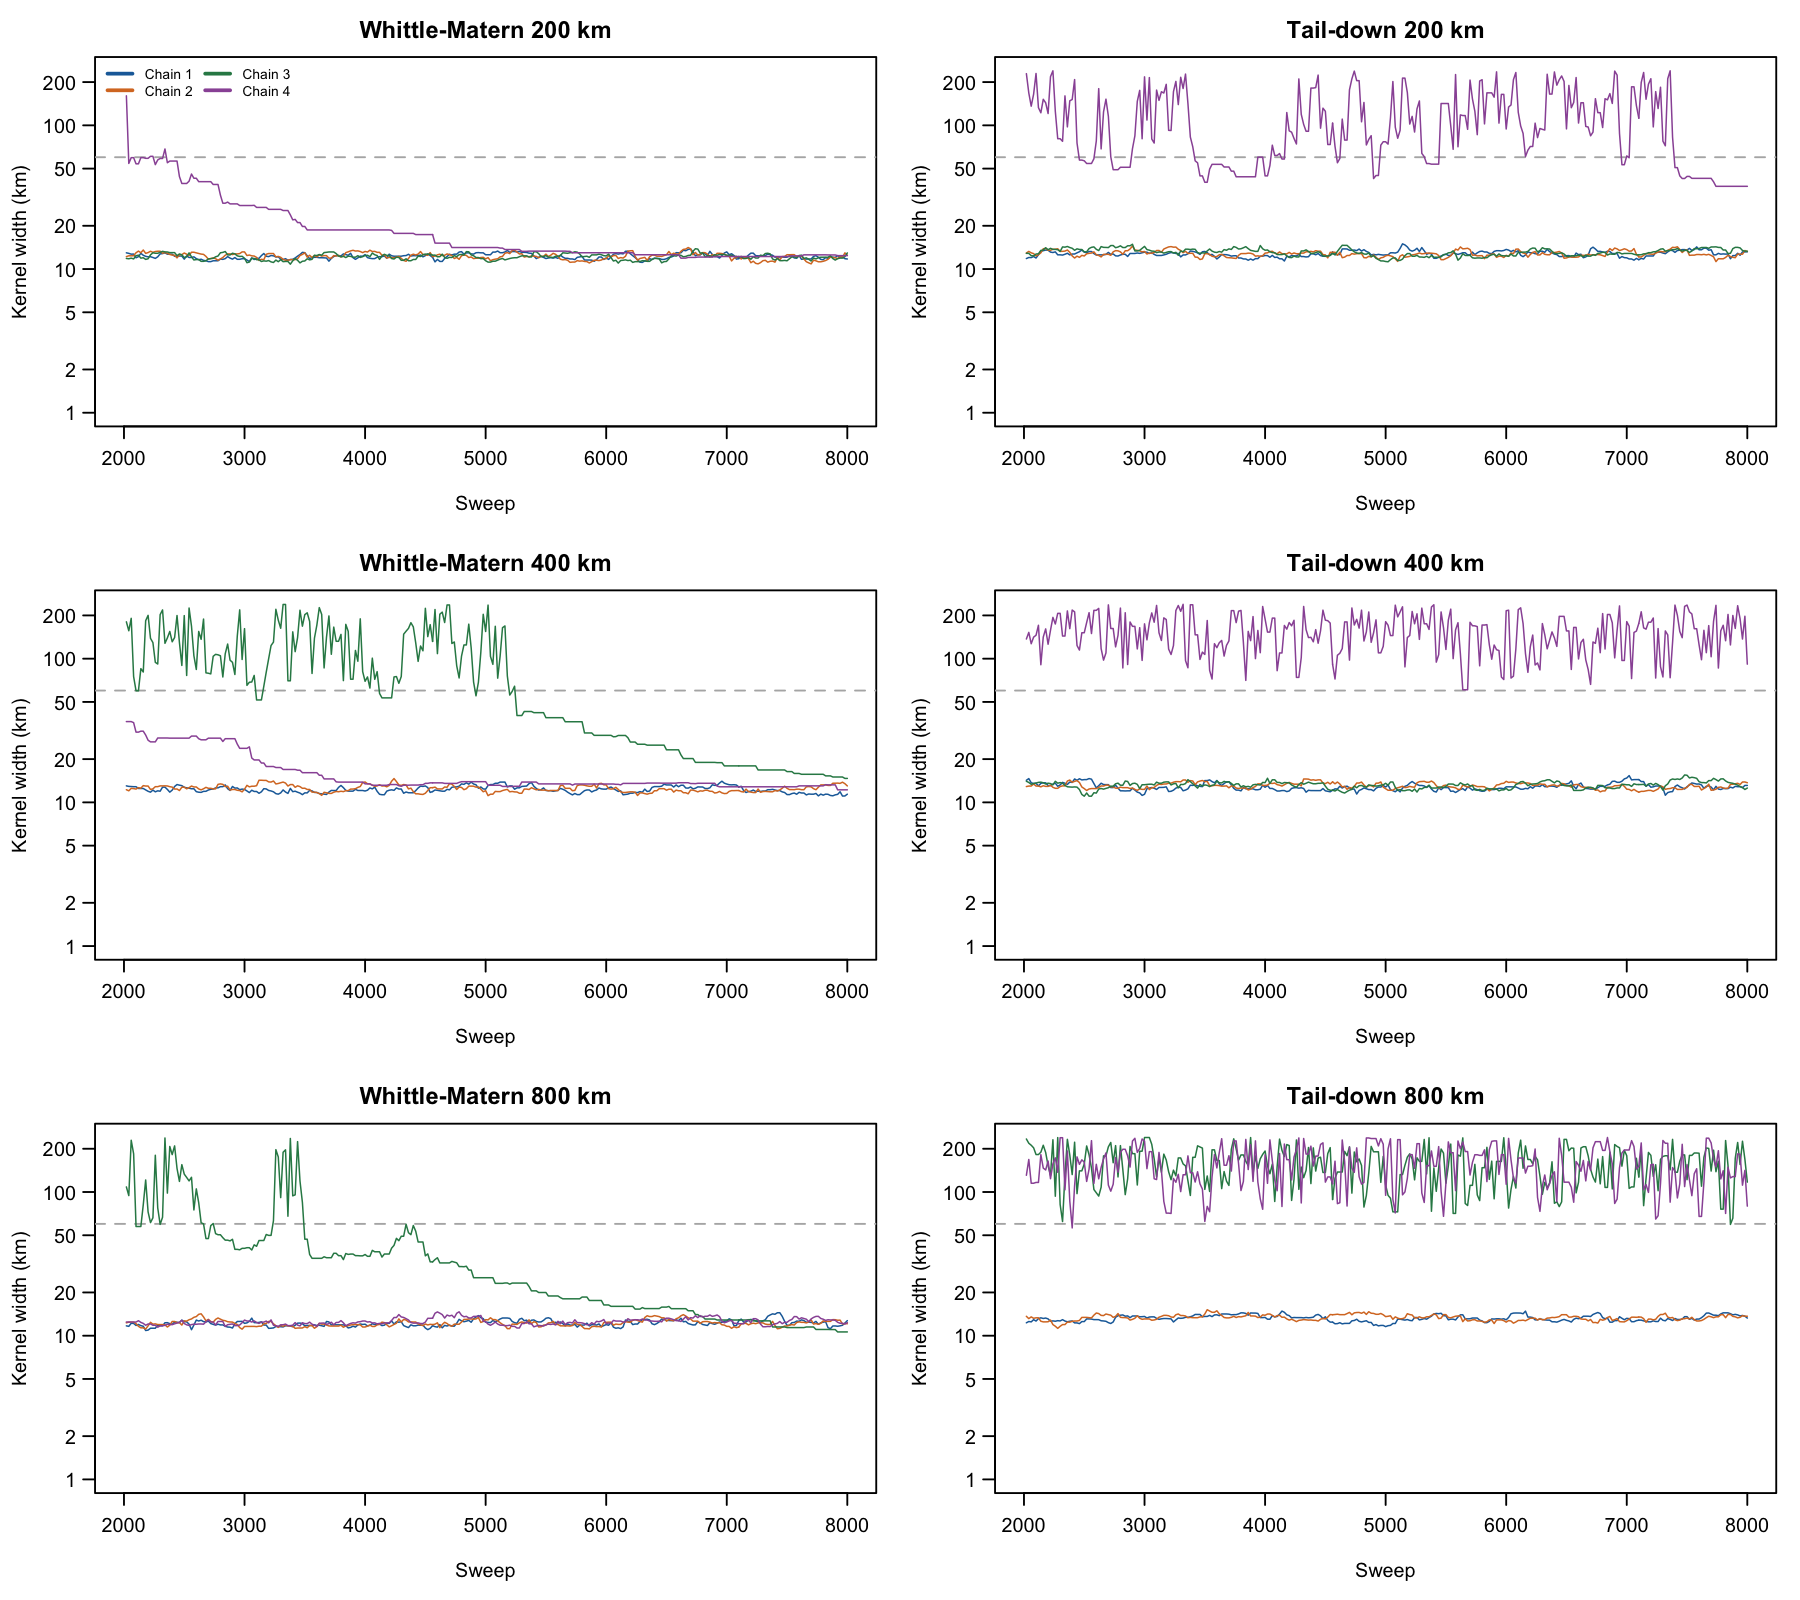
\includegraphics[width=.88\textwidth]{width_traces.png}
\caption{Full-data kernel-width traces after burn-in, shown every 20 sweeps. Colors distinguish the four chains, the vertical scale is logarithmic, and the dashed line marks the fixed 60~km cutoff.}
\label{fig:widths}
\end{figure}

\FloatBarrier
\subsection{Mixing of the latent Gaussian field}\label{sec:field-mixing}

The archived fits retain coefficient draws and running cell summaries, but no trajectories of $g$. We therefore replayed the four full-data chains for the tail-down model at $r=800$~km, using the revised code and the same 8,000-sweep schedule, 2,000-sweep burn-in, seeds and initial widths as the archived analysis. The field starts at zero in every chain; the initial widths are 10, 20, 40 and 80~km. The monitoring records values after both field colours have been updated, without changing proposals or random-number draws. Retained parameter draws agree with the archive to within $1.3\times10^{-14}$, and the stored cell summaries agree exactly.

We selected 128 vertex IDs at evenly spaced positions in the sorted list of vertices touching the survey footprint, and 32 from its complement, before inspecting their trajectories. We also recorded cell-length-weighted averages of the interpolated field over the whole network, the survey footprint, and its northern and southern halves, together with the north--south difference. The halves are defined by the median latitude of footprint cells. Diagnostics use all 6,000 retained states per chain, giving 24,000 stored draws for each monitored quantity; these coordinates and summaries do not exhaust all 145,329 field dimensions.

The broad field summaries mix poorly: their rank-normalized $\widehat R$ values range from 1.63 to 2.25, with bulk ESS estimates between 5.0 and 6.7 (Table~\ref{tab:field-mixing}). For the survey-footprint mean, the average within-chain autocorrelation is 0.999 at lag one and 0.896 at lag 100. The traces in Figure~\ref{fig:field-mixing} show persistent drift and disagreement, so these small ESS values are diagnostic warnings rather than a basis for precise Monte Carlo uncertainty estimates.

Local coordinates also show substantial dependence: among the 128 monitored footprint vertices, the median $\widehat R$ is 1.136, the maximum is 1.564, and 127 exceed 1.01; median bulk ESS is 21.7. Outside the footprint, 31 of the 32 monitored vertices exceed 1.01. Consequently, the field diagnostics support the earlier warning about incomplete posterior exploration, including spatial averages that can mix much more slowly than an individual coordinate. All fields were initialized at zero, so this check does not establish robustness to dispersed field starts.

The small conditional blocks provide a plausible mechanism for slow movement on large spatial scales, while dependence between the field, site counts, breeding coefficients and dispersal width may also contribute. These runs do not separate those causes or compare alternative samplers; larger-scale or joint updates would require their own empirical mixing assessment.


\begin{table}[H]
\centering\small
\caption{Latent-field diagnostics for the additional tail-down 800~km run. ESS is calculated across four chains; autocorrelations at lags 1 and 100 are averaged over the four within-chain estimates. The last row selects the largest $\widehat R$ among the 128 monitored footprint vertices.}
\label{tab:field-mixing}
\begin{tabular}{lrrrrr}
\toprule
Field quantity & $\widehat R$ & Bulk ESS & Tail ESS & ACF(1) & ACF(100)\\
\midrule
Whole-network mean & 2.249 & 5.0 & 21.2 & 0.998 & 0.839 \\
Survey-footprint mean & 1.703 & 6.3 & 13.8 & 0.999 & 0.896 \\
Northern mean & 1.998 & 5.4 & 11.6 & 0.999 & 0.882 \\
Southern mean & 1.629 & 6.7 & 20.3 & 0.999 & 0.865 \\
North--south contrast & 1.642 & 6.6 & 46.9 & 0.998 & 0.817 \\
Largest local $\widehat R$ & 1.564 & 7.3 & 18.3 & 0.954 & 0.536 \\
\bottomrule

\end{tabular}
\end{table}

\begin{figure}[htbp]
\centering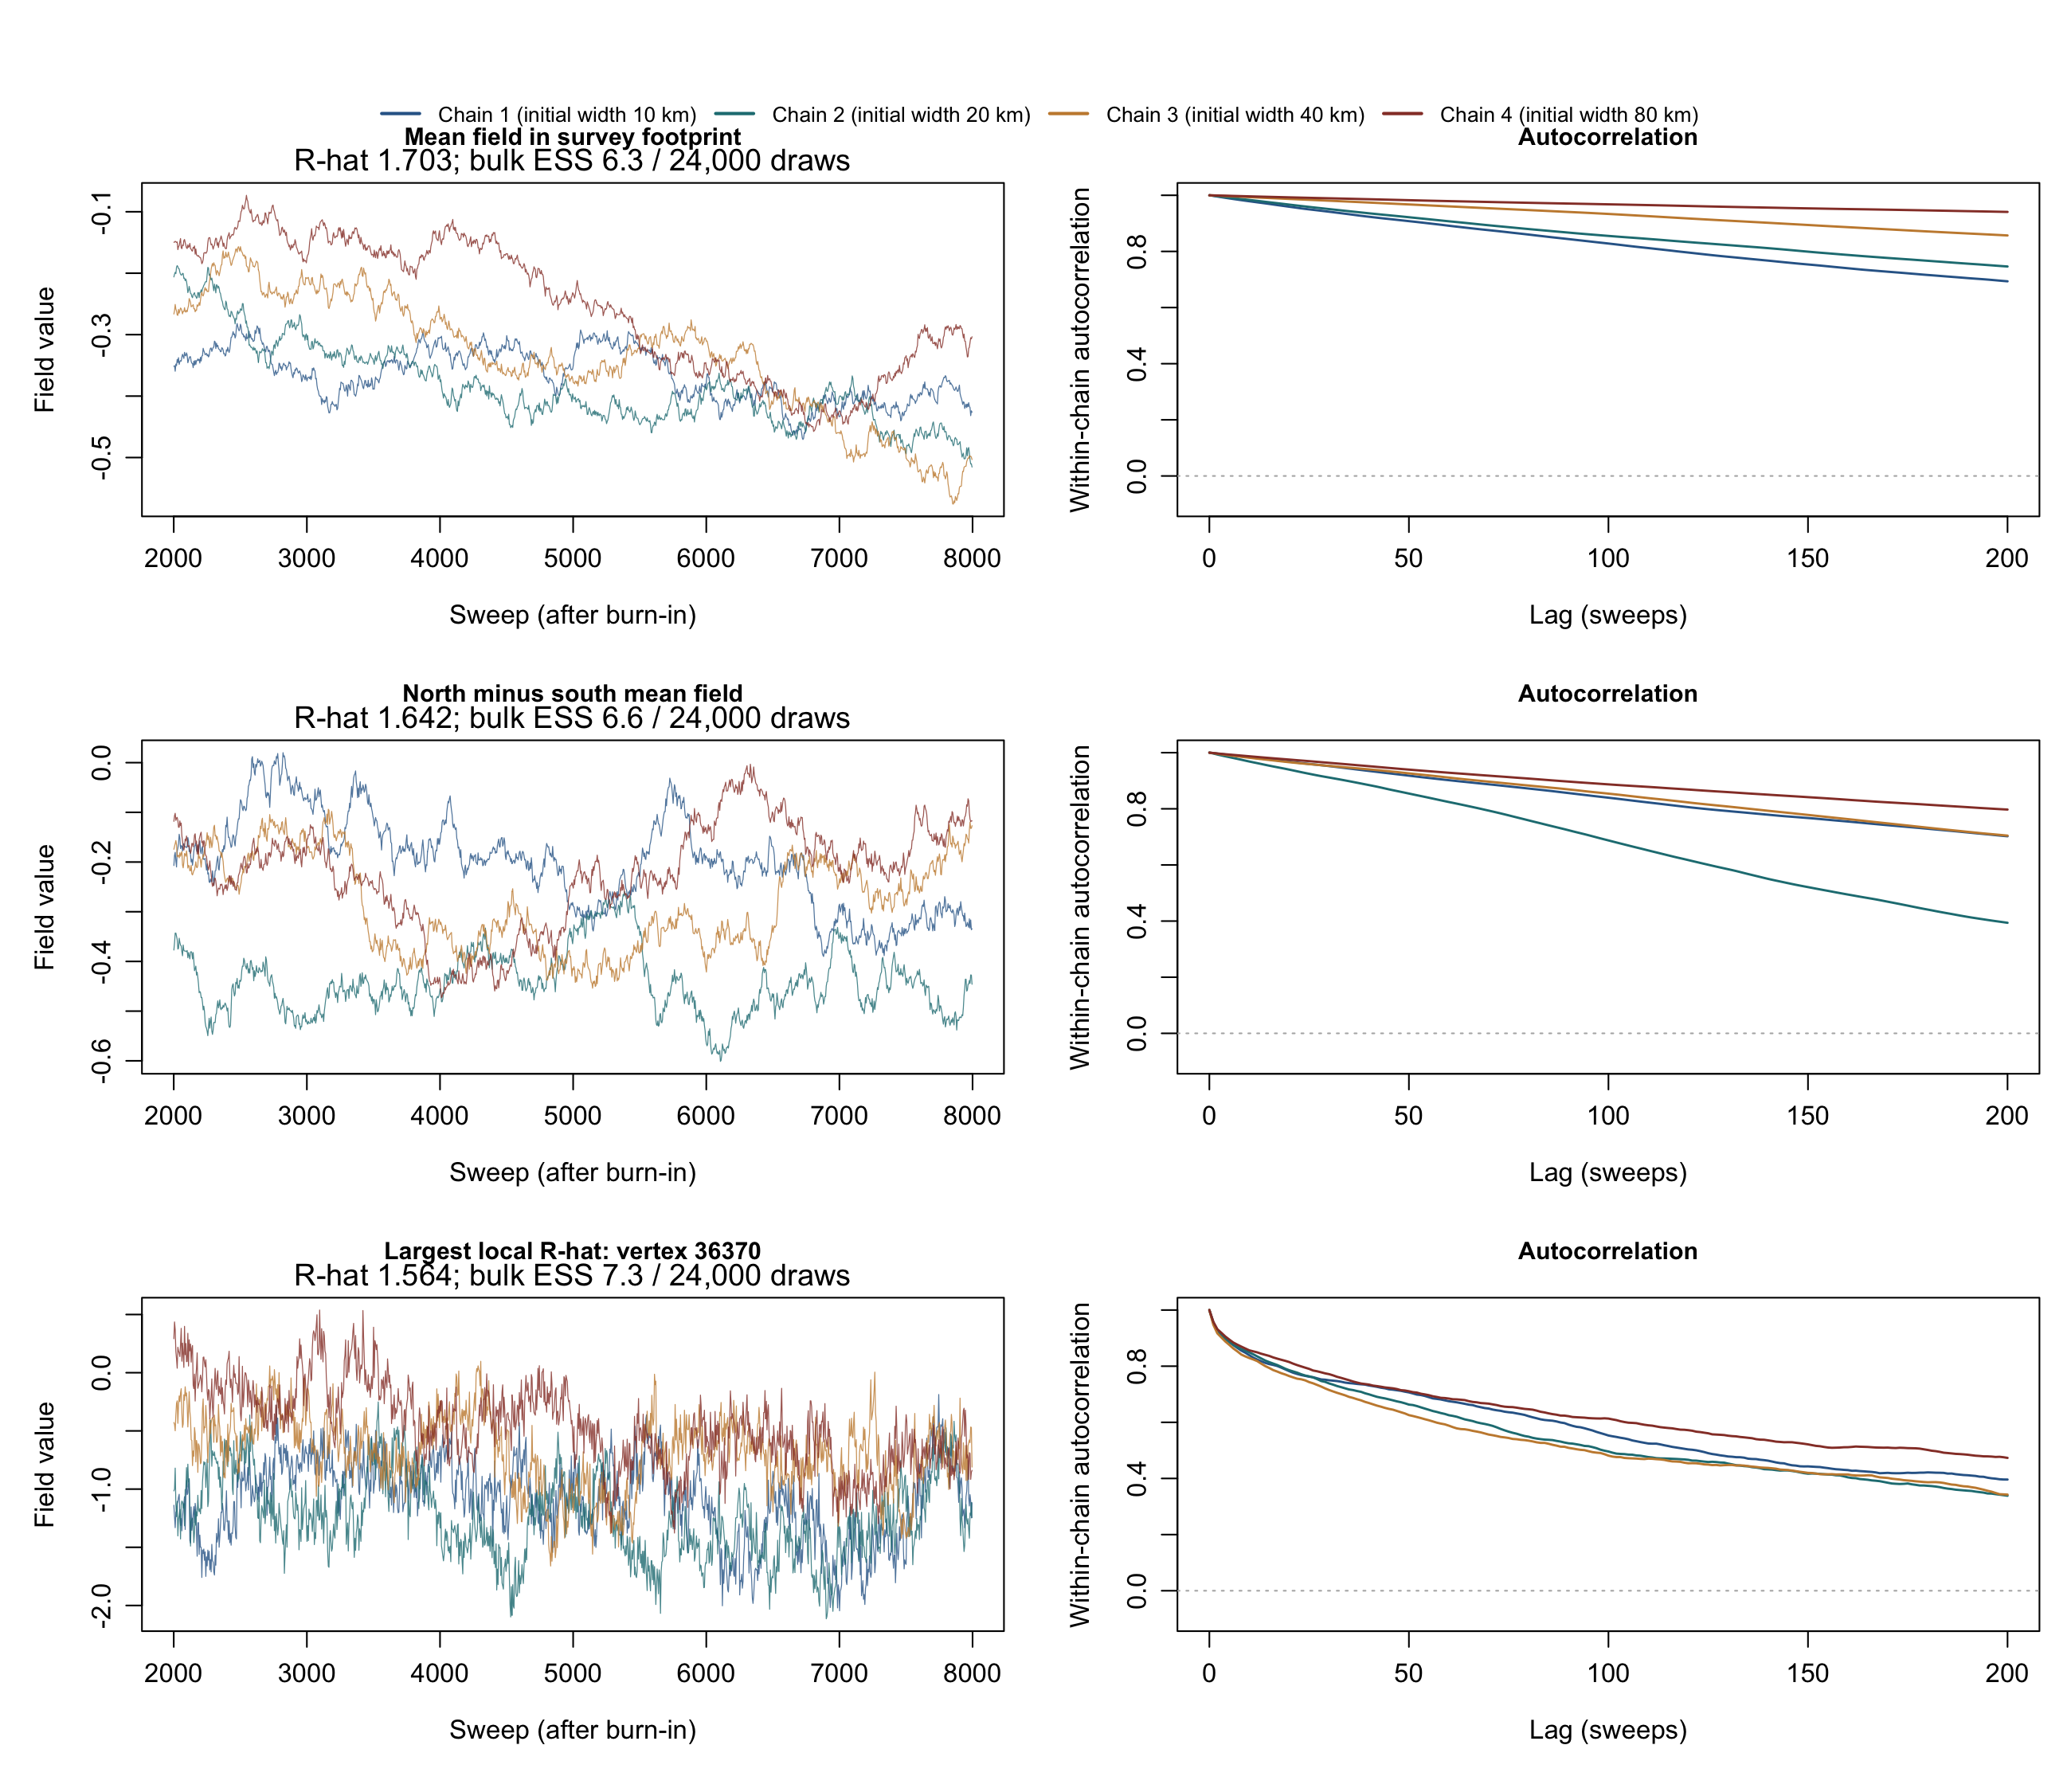
\includegraphics[width=\textwidth]{field_mixing.png}
\caption{Retained field traces and within-chain autocorrelations for the survey-footprint mean, the north--south contrast, and the monitored footprint vertex with the largest $\widehat R$. Colours identify the four chains; traces are displayed every fifth sweep, while all retained draws enter the diagnostics and autocorrelations.}
\label{fig:field-mixing}
\end{figure}
\FloatBarrier


\subsection{Fresh-landscape checks}

Table~\ref{tab:full} summarizes the full-data runs and their regenerated landscapes. The simulated overall positive fraction is above the observed 6.31\% in every configuration. Some settings also generate appreciably more nonzero villages than observed. These discrepancies warrant model and prior sensitivity analysis, alongside improved mixing; they cannot be resolved by interpreting a favorable held-out score as proof that the entire generative model is calibrated.

\begin{table}[H]
\centering\small
\caption{Exploratory full-data summaries. Width intervals are pooled 2.5\%--97.5\% quantiles; the final columns are means over fresh landscapes. Observed: 350 nonzero villages and 6.31\% positive.}
\label{tab:full}
\begin{tabular}{lrrrrr}
\toprule
Field & $r$ (km) & Width median & Width interval & Nonzero & Positive (\%)\\
\midrule
Whittle--Mat\'ern & 200 & 12.4 & 11.2--40.6 & 351.8 & 8.17 \\
Tail-down & 200 & 13.2 & 11.8--207.8 & 366.1 & 8.72 \\
Whittle--Mat\'ern & 400 & 13.2 & 11.4--187.9 & 358.1 & 8.26 \\
Tail-down & 400 & 13.3 & 11.9--219.4 & 378.0 & 9.65 \\
Whittle--Mat\'ern & 800 & 12.4 & 11.3--84.7 & 362.0 & 9.07 \\
Tail-down & 800 & 35.7 & 12.3--233.8 & 400.6 & 10.98 \\
\bottomrule

\end{tabular}
\end{table}

\FloatBarrier
\section{Code performance and validation}

The 10 November revision removes dense row extraction when initializing feasible source counts: the transposed sparse kernel lists only cells in reach of each positive village. It also reuses Poisson means between field summaries and the next count sweep, and skips the binomial calculation when a village has zero likelihood weight. The activity likelihood is still evaluated whenever its state is observed. Kernel construction now handles very broad and very narrow Gaussian widths without squaring the width or subtracting nearly equal probabilities. If a positive village has no representable positive kernel weight, initialization gives a direct error explaining the width and cell-resolution issue.

The code separates fixed design construction, initial counts, field updates and kernel updates into named functions and files. Comments identify the conditional distributions and the order of each sweep, including where all updates share the same exposure. These changes retain the existing public arguments and output structure.

A full-network benchmark used the same 900 villages, 286,068 cells, 145,329 field vertices, covariates, seed and sampler settings before and after the revision. Each run used 300 sweeps, including 100 burn-in sweeps, with marked sources, occurrence, relocation and a sampled Gaussian width; four repetitions were made per version in separate R processes. Median elapsed time fell from 12.677 to 11.431 seconds, a 9.8\% reduction in time (1.11 times as fast). Machine load affects these measurements. The retained outputs agreed with the previous implementation to a comparison tolerance of $10^{-11}$.

The full package test suite passed 970 assertions in 66 cases, with no test failures, skips or test warnings. Eighteen new assertions cover extreme Gaussian widths, normalization, feasible initialization, unsupported positive surveys and masked occurrence predictors. Separate direct-integration examples checked the unmarked count posterior, marked counts and spread, occurrence, and the conditional width update. For the latter, the sampled mean log width and width differed from quadrature by 0.48 and 0.29 estimated Monte Carlo standard errors, respectively. Package checking completed with zero errors, three warnings and one note; these concern existing REMO character encoding and documentation of non-LGCP arguments. The development loader also reports the REMO encoding warnings outside the test results.


These timings concern computation for a short fixed workload, including initialization; they do not measure effective independent draws per second. The speed improvement does not resolve the chain disagreement in the archived scientific analyses. The original full-data comparisons and 120 holdout chains were not rerun for the performance benchmark; the separate field-diagnostic refit is described in Section~\ref{sec:field-mixing}.

\section{Discussion}

The LGCP provides an explicit account of shared, unobserved breeding sites and their contributions to village exposure. For the saved held-out forecasts, the tail-down field at 800~km gives the best aggregate scores among the six configurations. The strongest limitation is posterior exploration: width regimes disagree across chains, and many local predictions also have poor diagnostics. Site-density assumptions, mark contrast and transmission regression may compensate for one another, making source-rate sensitivity and better exploration of width particularly relevant.

A subsequent scientific comparison should retain the same folds and score definitions, improve mixing, and assess cell-resolution and fixed-hyperparameter sensitivity. The current implementation checks support the tested calculations and provide a faster starting point. They do not turn the archived finite-chain rankings into a settled model-selection result.

\appendix
\section{Files and reproducibility}

The directory \path{inst/reports/lgcp/data} contains the numerical summaries, village forecasts, survey coordinates, thinned width traces and field-diagnostic plotting data. The original full-data and spatial holdout archives and the separate field-monitoring run, including the source files for every bundled table, are listed in \texttt{data/sources.txt}. The figures and tables can be rebuilt from the repository root with
\begin{verbatim}
Rscript inst/scripts/lgcp/report_figures.R
cd inst/reports/lgcp
pdflatex -halt-on-error lgcp_river_model.tex
bibtex lgcp_river_model
pdflatex -halt-on-error lgcp_river_model.tex
pdflatex -halt-on-error lgcp_river_model.tex
\end{verbatim}
The performance script is \texttt{inst/scripts/lgcp/benchmark.R}. Source snapshots, timings, numerical replay checks, test logs and package-check output for the code revision are retained in \texttt{jonas\_local/lgcp\_audit\_20261110}. Scientific tables are reconstructed from the bundled village forecasts; their generation checks that the aggregate Brier, CRPS and log scores agree with the archived comparison.

\bibliographystyle{plainnat}
\bibliography{references}

\end{document}
